\section{Assessment and Management of Data Quality}
These instruments, however, are prone to data quality issues due to
the challenging operating conditions in field, sensor failures, need for
recalibration etc. ARM Data Quality Office, established in year 2000,
coordinates detection and reporting of data quality for all datastreams.
Data Quality Reports (DQR) can be submitted by data quality analysts,
instrument mentors, facilities operations personnel or data users and
are saved within a consistent and searchable PostgreSQL database.
However, with large numbers of instruments and streaming datastream
maintained by the program, DQRs can be frequent and many. 
Figure~\ref{fig:dqr_by_instrument} shows the reported data quality
issues for 20 ARM instruments over time. 

\begin{figure*}
 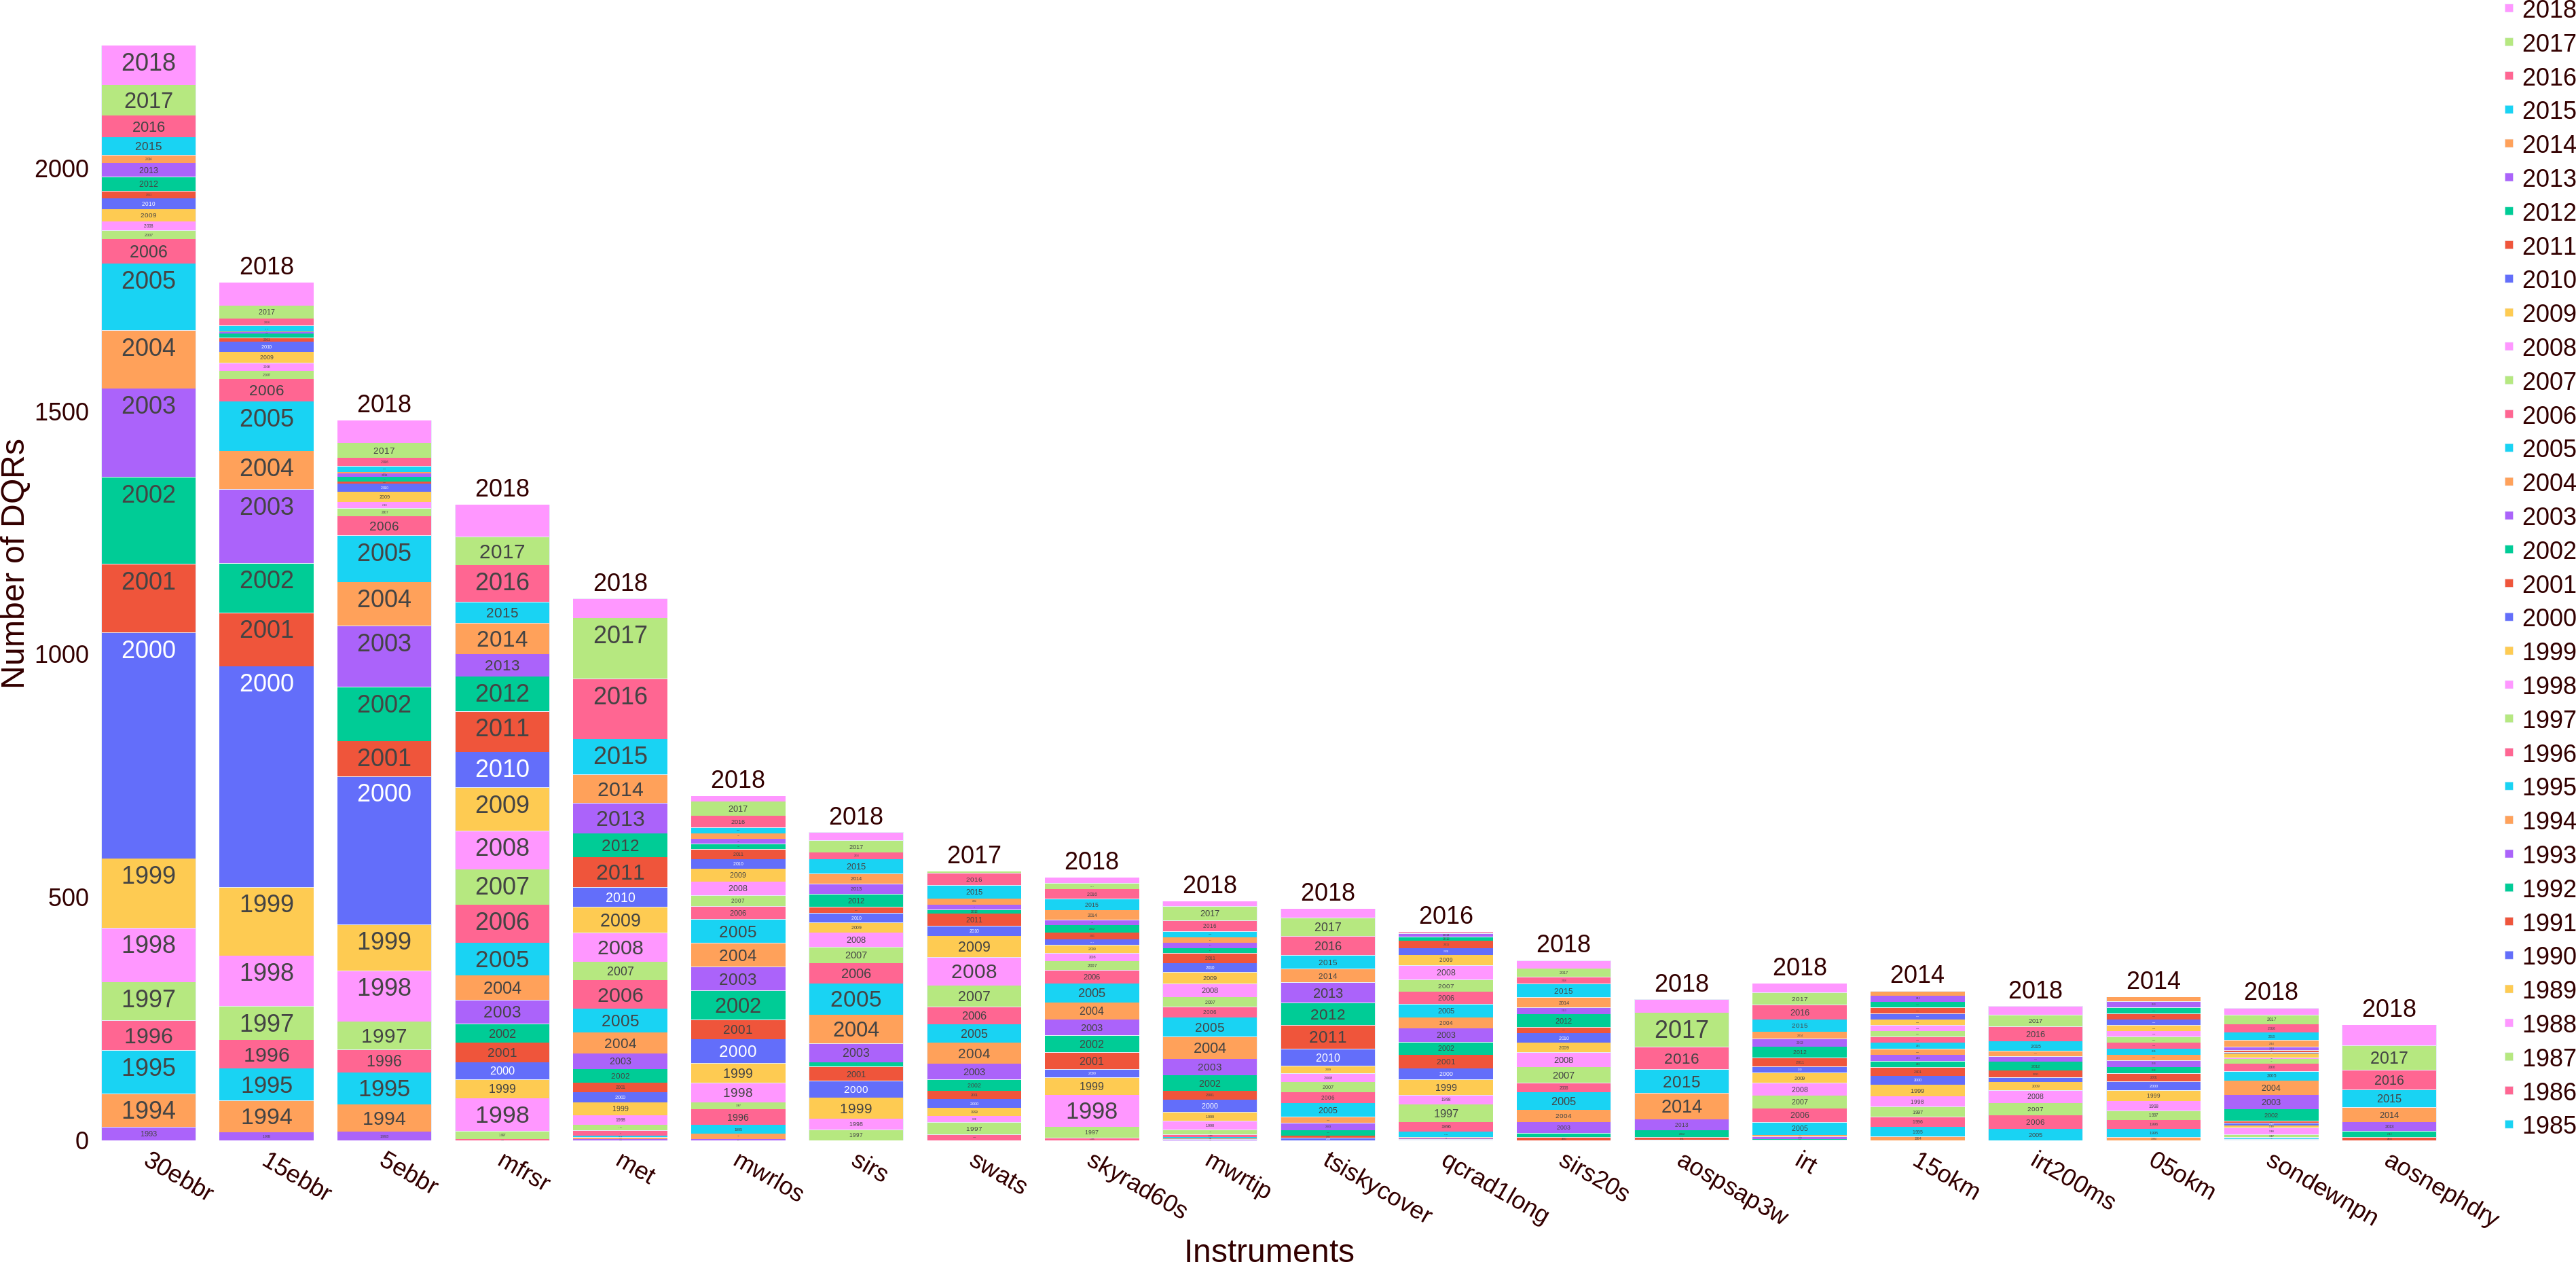
\includegraphics[width=\linewidth]{figures/dqr_by_instrument_20.png}
 \caption{DQRs for select 20 instruments over the period 1993-2019 show
	 that some instruements are more prone to data quality issues than
		 the others.}
 \label{fig:dqr_by_instrument}
\end{figure*}

\begin{figure*}
 \subfloat[30 EBBR]{
  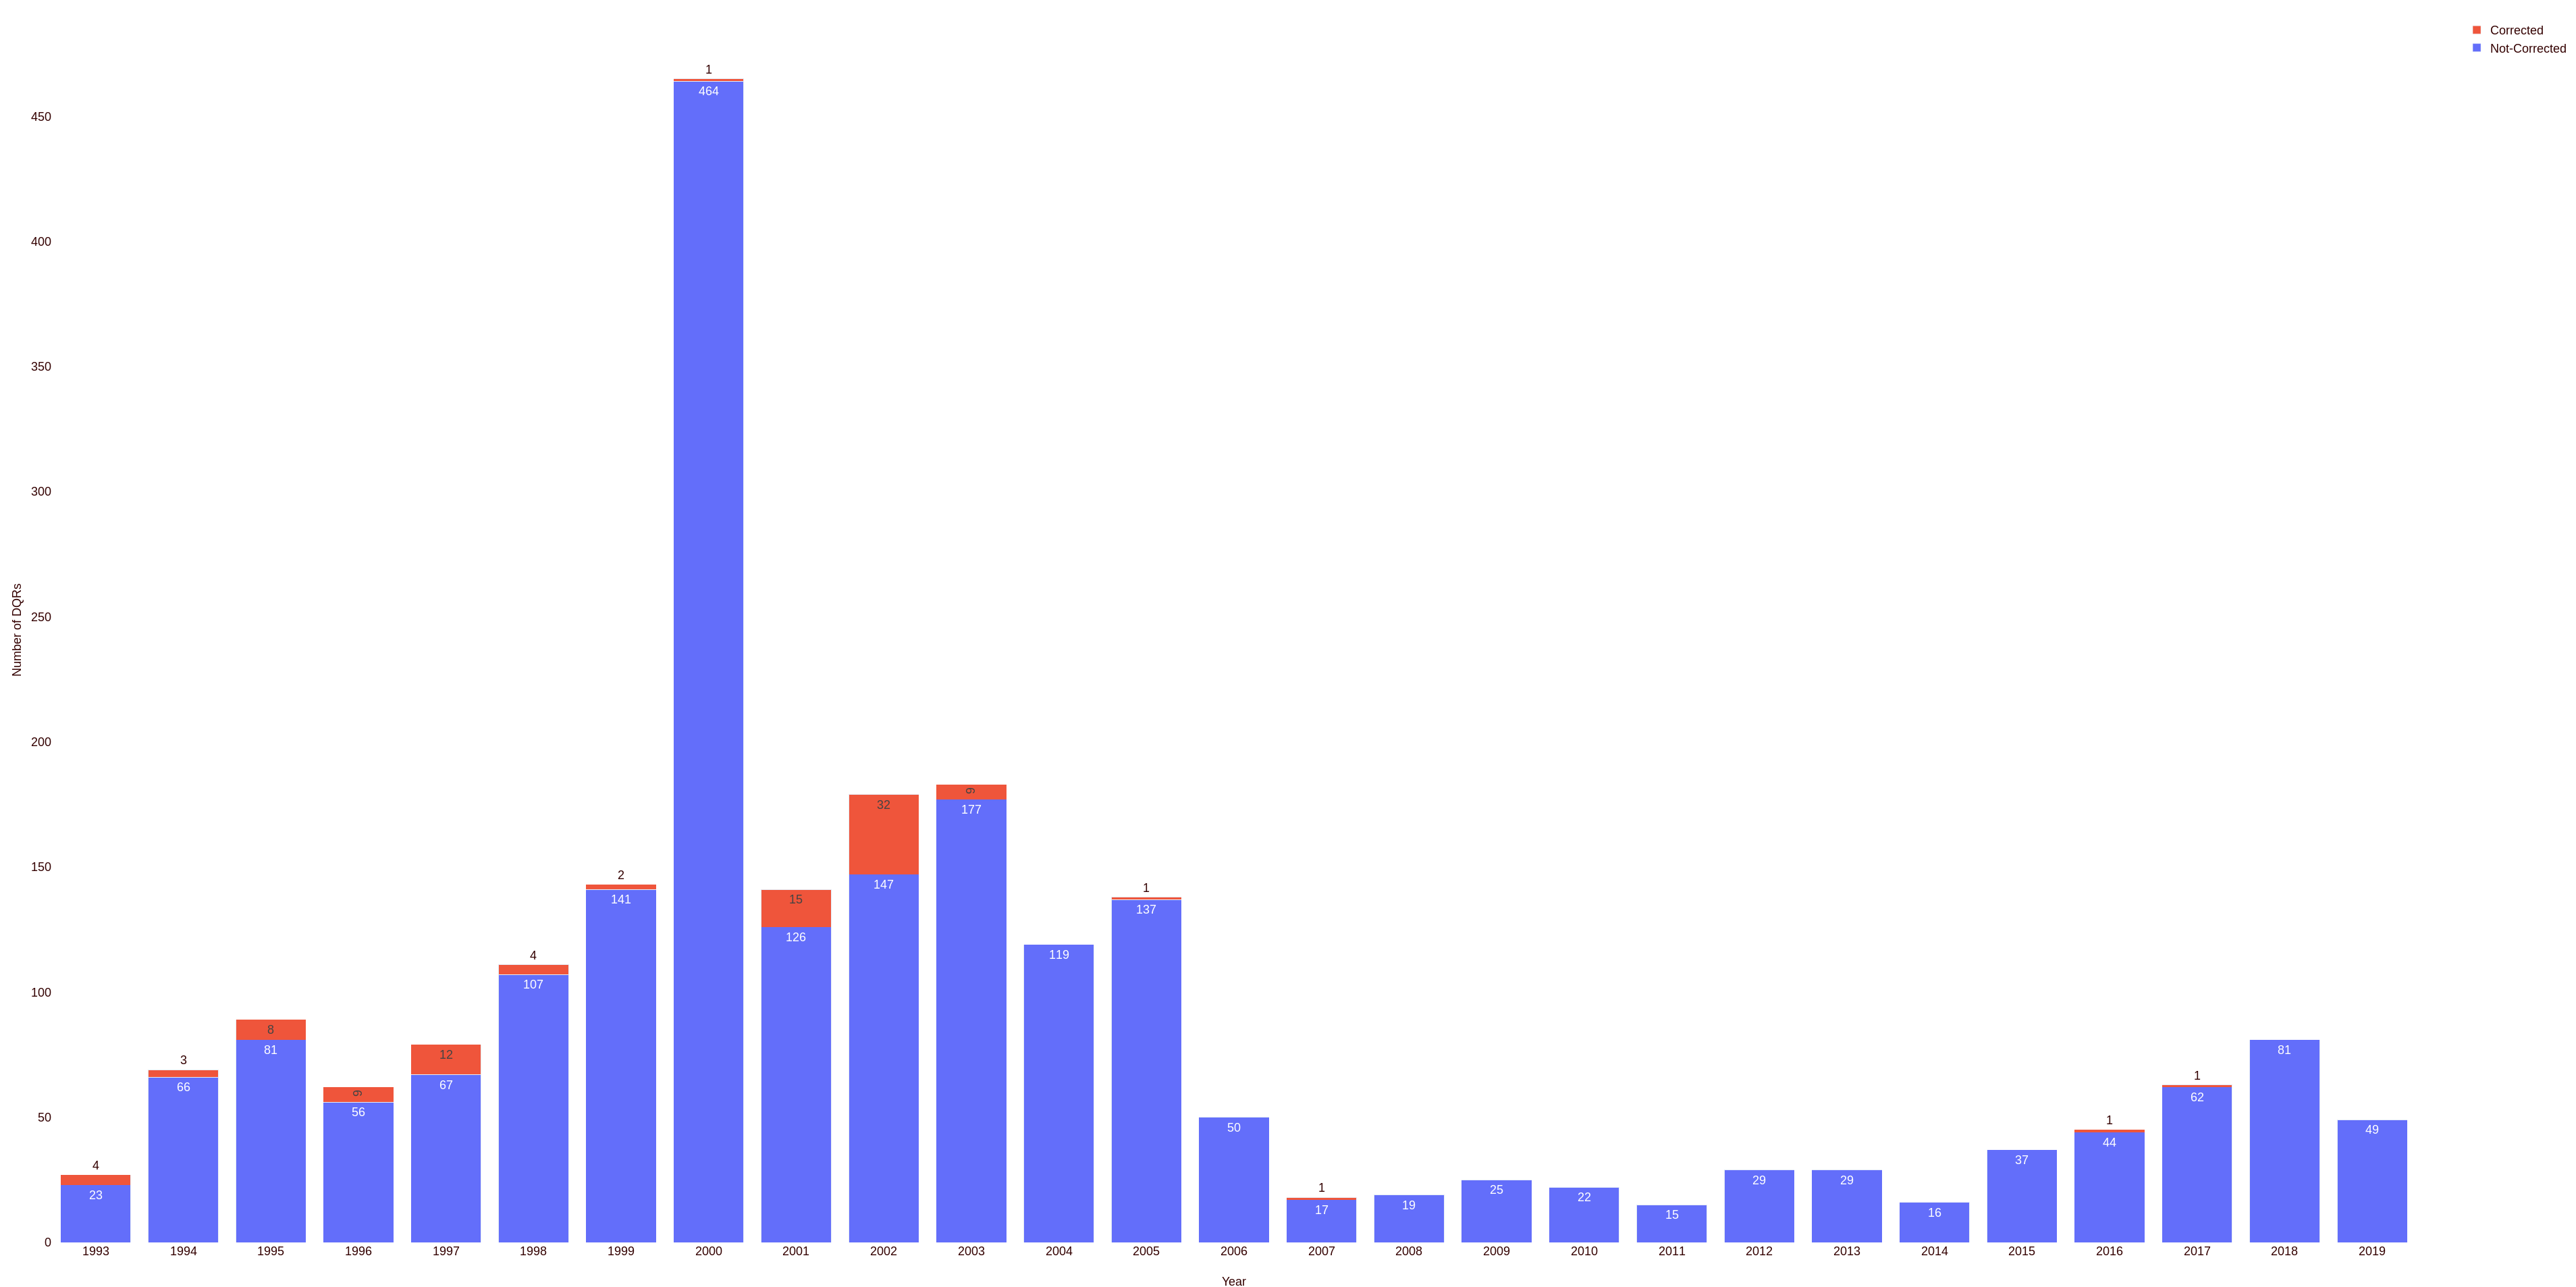
\includegraphics[width=0.33\linewidth]{figures/30ebbr_dqr_reproc_by_year.png}
 }
 \subfloat[MET]{
  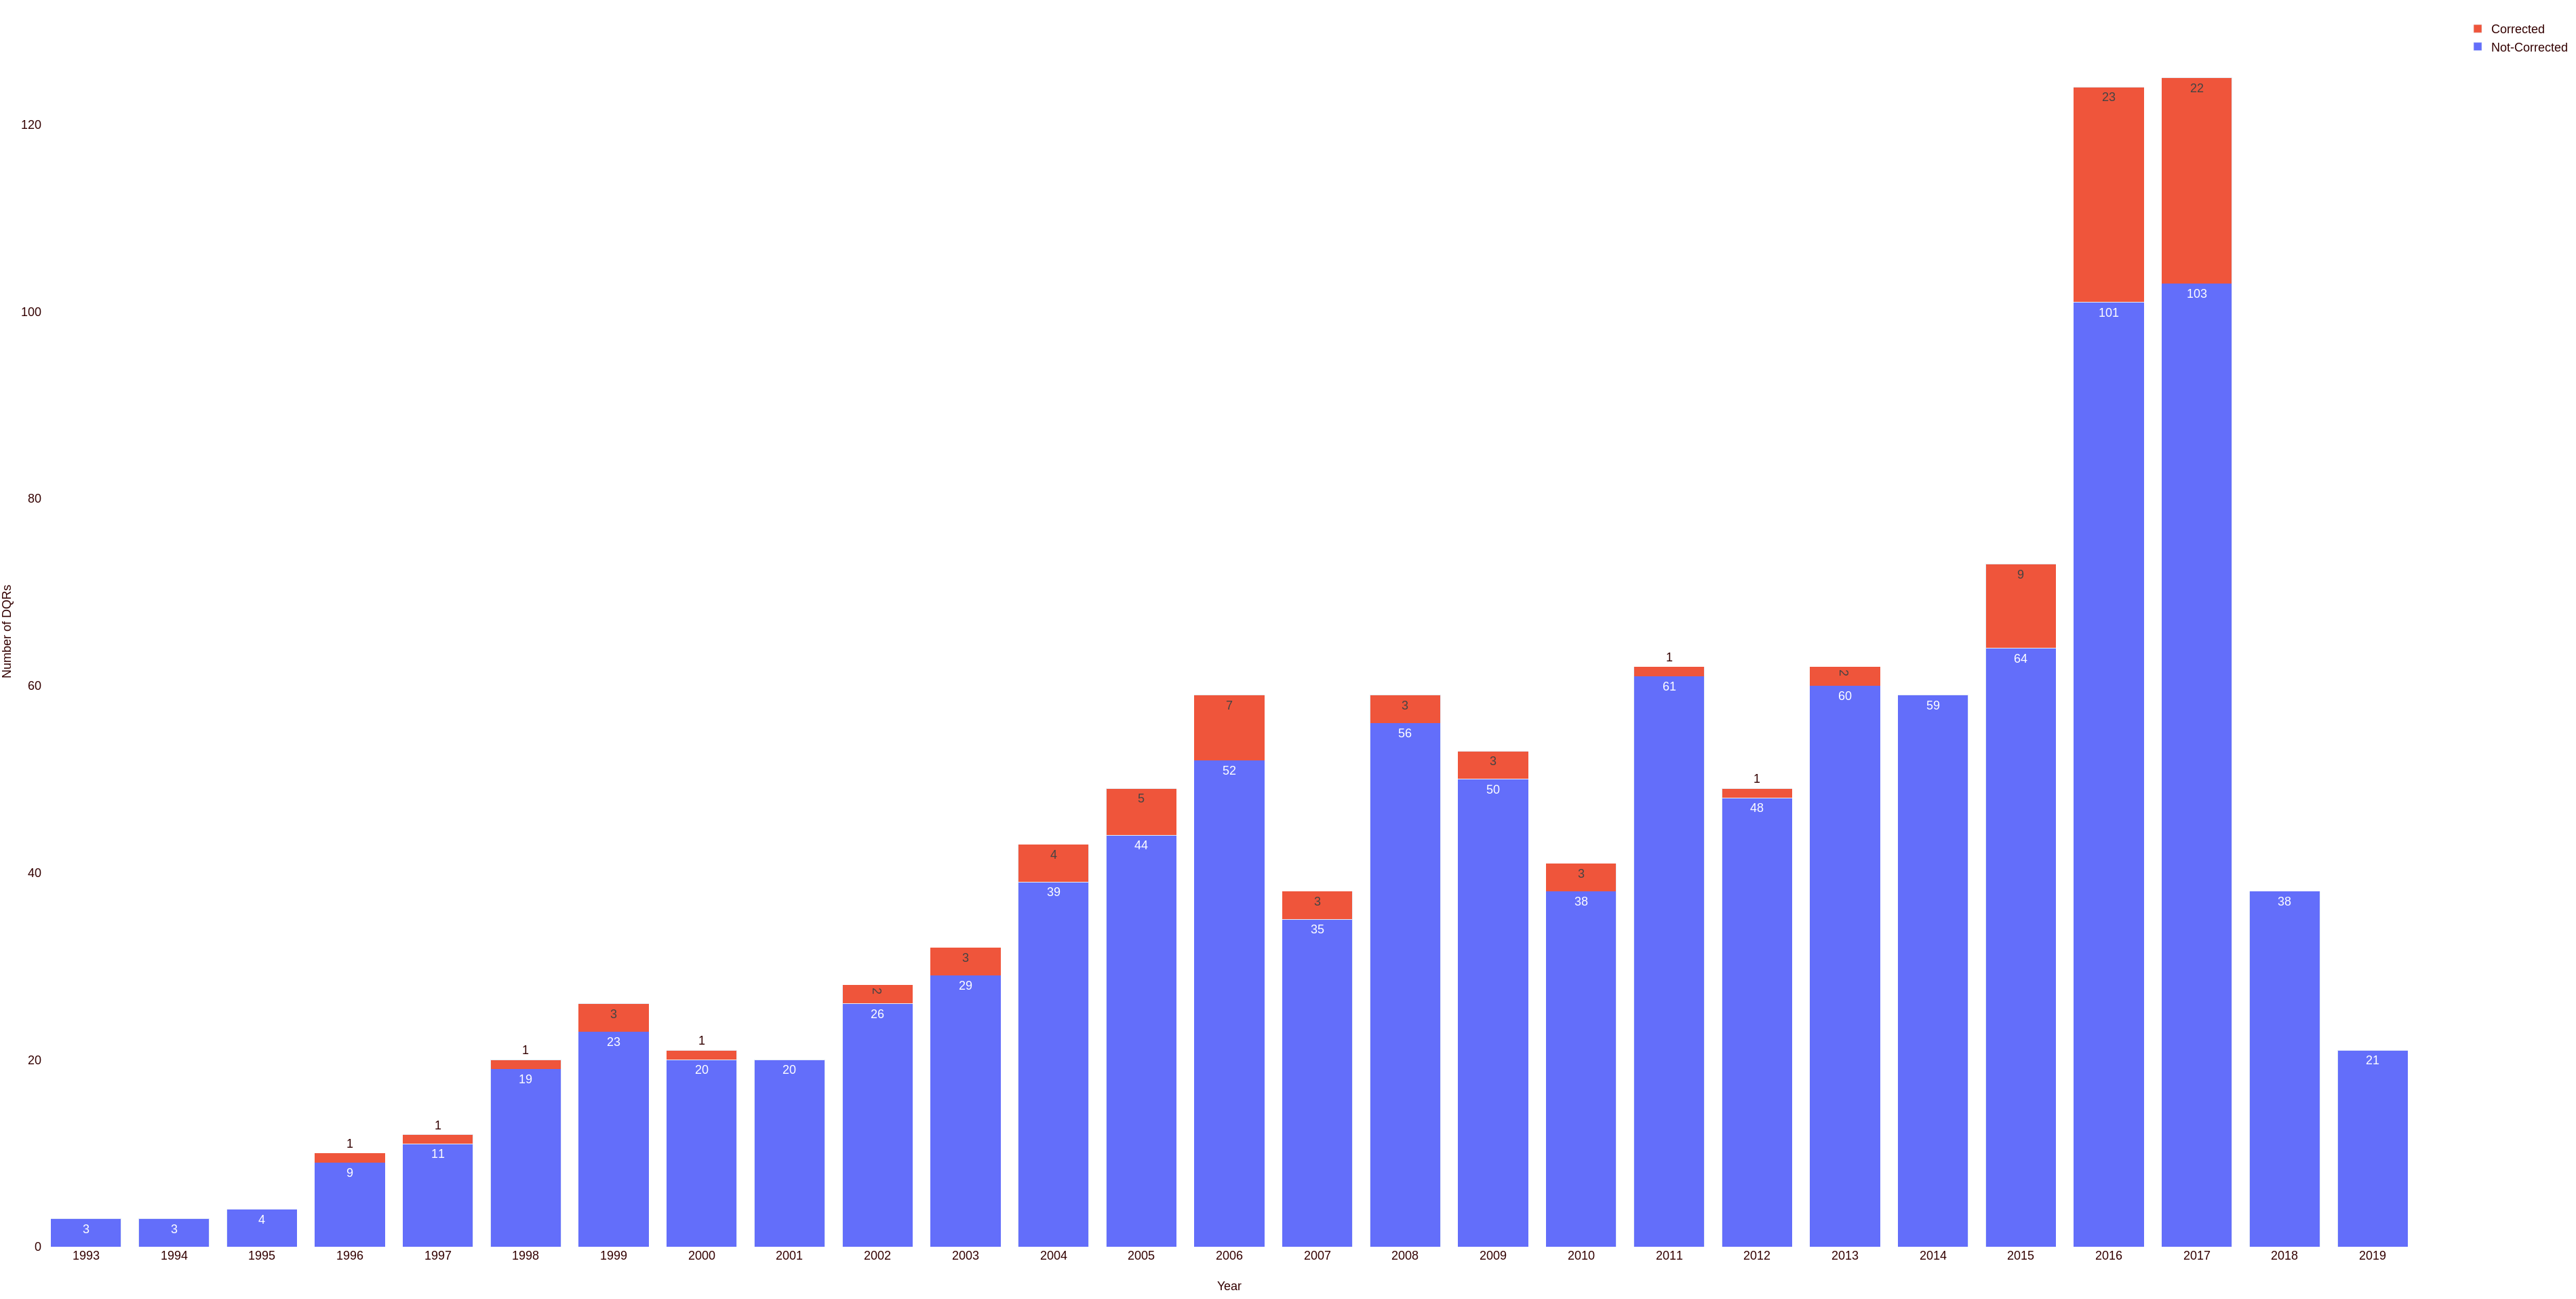
\includegraphics[width=0.33\linewidth]{figures/met_dqr_reproc_by_year.png}
 }
 \subfloat[RADFLUX]{
  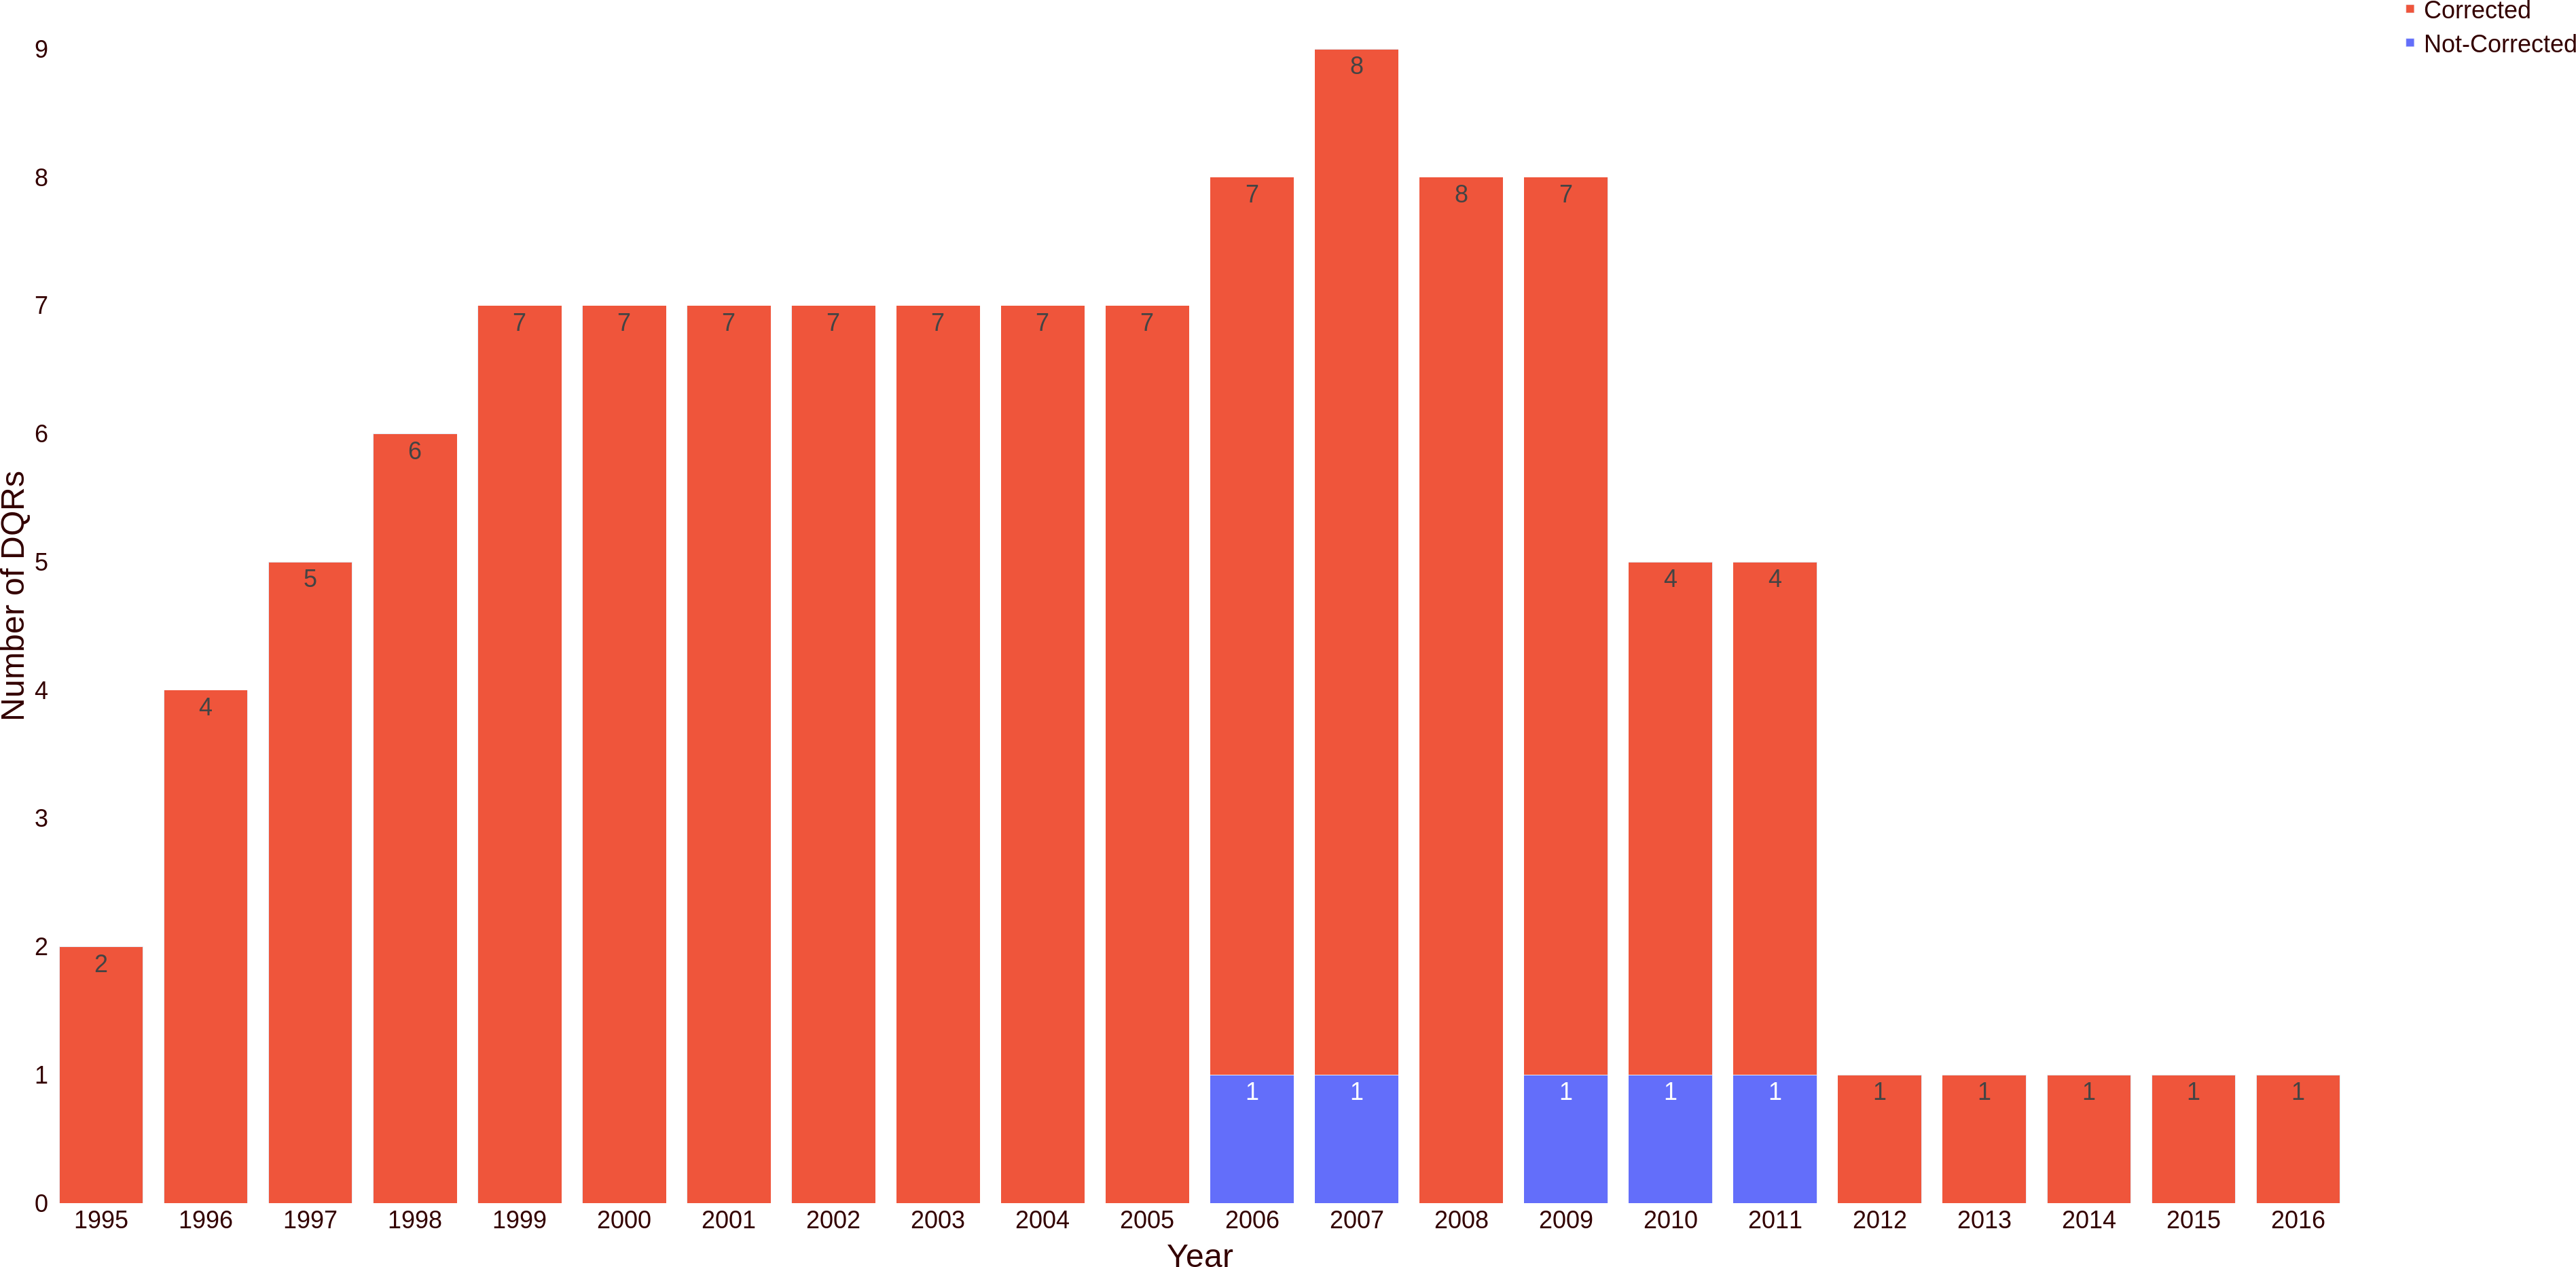
\includegraphics[width=0.33\linewidth]{figures/radflux_dqr_reproc_by_year.png}
 }
 \caption{DQRs for select 20 instruments over the period 1993-2019 show
	 that some instruements are more prone to data quality issues than
		 the others.}
 \label{fig:dqr_instrument_per_year}
\end{figure*}
